\documentclass[pdflatex, sn-basic]{sn-jnl}

%% --- Packages and commands from main.tex ---

\usepackage{lmodern}
\usepackage{microtype}
\usepackage{anyfontsize} % Helps with some font size scaling issues
\usepackage{exscale} % Helps scale math fonts correctly
\setlength{\marginparwidth}{2cm}
\usepackage{todonotes}
% Typeset todo notes ragged right. The class's \raggedright zeroes \parfillskip
% and leaks into tikz's ragged modes via \pgfutil@raggedright, so the plain
% align=left (finite 2em stretch) leaves every note line underfull; "flush left"
% keeps the 1fil \rightskip and typesets the note boxes without warnings.
\tikzset{notestyleraw/.append style={align=flush left}}
% The unbreakable inline todo boxes leave pages that cannot stretch to the full
% text height under the class's \flushbottom (underfull \vbox warnings);
% drop this once the todos are gone.
\raggedbottom
% sn-jnl's running heads (\ps@headings, \ps@titlepage) put an empty \hbox after
% \vspace*{-48pt} inside a \vbox to 0pt, which cannot stretch back to size and
% triggers an underfull \vbox on every shipout. The heads are empty anyway;
% rebuild the page styles without the broken boxes, keeping the same footers.
\makeatletter
\def\ps@headings{%
    \def\@oddfoot{\hfill\thepage\hfill}%
    \let\@evenfoot\@oddfoot%
    \let\@oddhead\@empty%
    \let\@evenhead\@empty%
    \let\@mkboth\markboth}%
\def\ps@titlepage{%
    \let\@oddhead\@empty%
    \let\@evenhead\@empty%
    \def\@oddfoot{\vbox to 18pt{\vfill\reset@font\rmfamily\hfil\thepage\hfil}}%
    \def\@evenfoot{}}%
\makeatother
\pagestyle{headings}

\usepackage{amsmath}
\usepackage[british]{babel}
\usepackage[english=british]{csquotes}

\usepackage{tikz}
\usepackage{pgfplots}
\pgfplotsset{compat=1.18}
\usepgfplotslibrary{fillbetween}
\usepgfplotslibrary{groupplots}
\usepgfplotslibrary{external}
\tikzexternalize[prefix=tikz/]
\tikzset{external/mode=graphics if exists}

\usetikzlibrary{patterns, arrows.meta, decorations.pathreplacing, calligraphy}

\usepackage[outline]{contour}
\contourlength{1.8pt}

\usepackage{acro}

\RenewAcroTemplate{long-short}{%
\acroiffirstTF{%
\acrowrite{long}%
~(%
\acroifT{foreign}{\acrowrite{foreign},~}%
\acrowrite{short}%
\acroifT{alt}{~\acrotranslate{or}~\acrowrite{alt}}%
\acrogroupcite )%
}%
{\acrowrite{short}}%
}


% ========================================
% Theorem-like environments
% ========================================

\theoremstyle{thmstylethree}% class style: bold head, upright body
\newtheorem{hypothesis}{Hypothesis}

% ========================================
% Hyphenation
% ========================================

\hyphenation{mo-ritz block-chain na-ka-mo-to crypto crypto-cur-ren-cy crypto-cur-ren-cies main-net}

% ========================================
% Acronyms
% ========================================

\acsetup{
    single-style = long,
    single       = true
}

\DeclareAcronym{SEC}{
    short = SEC,
    long  = United States Securities and Exchange Commission
}

\DeclareAcronym{HFT}{
    short = HFT,
    long  = high-frequency trading
}

\DeclareAcronym{ICT}{
    short = ICT,
    long  = information and communications technology
}

\DeclareAcronym{DeFi}{
    short = DeFi,
    long  = decentralised finance
}

\DeclareAcronym{TradFi}{
    short = TradFi,
    long  = traditional finance
}

\DeclareAcronym{MEV}{
    short = MEV,
    long  = maximal extractable value
}

\DeclareAcronym{CEX}{
    short = CEX,
    long  = centralised exchange
}

\DeclareAcronym{DEX}{
    short = DEX,
    long  = decentralised exchange
}

\DeclareAcronym{L1}{
    short = L1,
    long  = layer 1 blockchain
}

%\def\querybox#1{\protect\fboxsep=0pt\colorbox{yellow}{#1}}

\def\mystar{\relax}

\def\tciLaplace{\mathcal{L}}
\def\dint{\mathop{\displaystyle \int}}%


\begin{document}
	\title[The Regressive Tax of Decentralisation]{The Regressive Tax of
	Decentralisation: Market Power and Distributional Inequality in Decentralised Exchanges}

	\author[1,2]{\fnm{Jana} \sur{Botkuljak}}
	\author[3]{\fnm{Natalie} \sur{Hlusi}}
	\author*[4,5]{\fnm{Francesco} \sur{Pierangeli}}\email{f.pierangeli@bham.ac.uk}
	\author*[6,7]{\fnm{Moritz} \sur{Platt}}\email{moritz.platt@kcl.ac.uk}

	\affil[1]{\orgname{University of Osijek}, \orgaddress{\city{Osijek}, \country{Croatia}}}
	\affil[2]{\orgname{Croatian National Bank}, \orgaddress{\city{Zagreb}, \country{Croatia}}}
	\affil[3]{\orgname{University of San Francisco}, \orgaddress{\city{San Francisco}, \state{CA}, \country{USA}}}
	\affil[4]{\orgname{University of Birmingham}, \orgaddress{\city{Birmingham}, \country{UK}}}
	\affil[5]{\orgname{University College London}, \orgaddress{\city{London}, \country{UK}}}
	\affil[6]{\orgname{King's College London}, \orgaddress{\city{London}, \country{UK}}}
	\affil[7]{\orgname{Google}, \orgaddress{\city{Mountain View}, \state{CA}, \country{USA}}}

	\abstract{Work in Progress.}

	\pacs[JEL Classification]{}

	\maketitle

\section{Introduction}
\label{sec:introduction}

\Ac{DeFi} was built on the promise of creating more open, transparent, and accessible financial markets. The same transparency that enables trust, however, also creates opportunities to exploit transaction ordering for profit. One of the most prominent examples is \ac{MEV}, defined as the profit obtainable through the strategic ordering, insertion, or exclusion of transactions within a block~\citep{Daian2020}. Among the various forms of \ac{MEV}, sandwich attacks are particularly important because they generate profits through direct value extraction from traders.

Existing research has significantly improved our understanding of the technical mechanisms underlying \ac{MEV}, including transaction-ordering, attack detection methods, and protocol-level mitigation strategies~\citep{Daian2020,Qin2022,Heimbach2022}. However, while the mechanics of extraction are increasingly well understood, considerably less attention has been paid to its distributional consequences. An important question therefore remains: who ultimately bears the cost of \ac{MEV} in decentralised markets? Understanding the distribution of these costs is critical for assessing whether decentralised markets deliver on their promise of creating fair and accessible financial systems.

This paper examines the distributional incidence of sandwich attacks on Ethereum during 2024--2025 using a large-scale dataset of detected sandwich activity. We analyse both the concentration of extraction among searchers and the allocation of losses across victim groups.

By shifting the focus from the mechanics of extraction to its economic incidence, this paper contributes to the growing literature on blockchain market microstructure and the broader consequences of financial innovation.


	\subsection{Mechanics of a Sandwich Attack}
	\label{subsec:mechanics}

	Central to \ac{MEV} is the concept of a \emph{mempool}, a cache of blockchain
	transactions proposals from which miners select transactions to include in
	blocks, typically prioritizing those that provide high rewards~\citep{Saad2019}.
	A sandwich attack consists of eight stages as shown in \autoref{fig:sandwich-attack}.
	% a) Monitor Mempool
	Attackers engaging in \ac{MEV} in general, and sandwich attacks in particular, continuously
	monitor transaction proposals admitted to those pools to detect \ac{MEV}
	opportunities~\citep{Prasath2024}.
	% b) Identify Victim
	Proposers of particularly large trades or liquidation transactions are
	promising victims~\citep{Weintraub2022}.
	% c) Submit Front-Run
	The attacker can use their knowledge of proposed transactions to execute a
	competing swap with a higher gas price, thereby increasing the likelihood of acceptance
	of their competing transaction, to front-run the victim~\citep{Stucke2022}.
	% d) Front-run executes
	If successful, the attacker's transaction is performed before the victim's transaction,
	leading to the victim suffering an objective loss due to the value difference
	from a fairly determined market price~\citep{Choi2024}.
	% e) Victim swap
	This unfavourable price, skewed by the front-running, presents a \enquote{tax} on
	the victim's trade, i.e., a victim would receive fewer tokens than anticipated
	due to the rise in token price induced by the front-run transaction~\citep{Heimbach2022}.
	% f) Submit back-run
	Following a successful front-run, an attacker may endeavour to execute a second
	transaction to counteract the effects of the previous transaction and to close out
	the earlier position~\citep{Zhao2025}. An attacker can execute such attack over
	two blocks where the back-run is sequenced as the first newly submitted swap in
	the second block~\citep{Baum2023}.
	% g) Back-run executes
	The execution of the back-run transaction finalizes the sandwich attack~\citep{Guidi2025}.
	% h) Victom loss
	With the successful execution of the attack, the victim realises a loss in the
	amount of the difference between the slippage tolerance and the actual price
	movement, which the attacker extracts as profit~\citep{Heimbach2022}.

	\begin{figure}[t]
		\centering
		\tikzsetnextfilename{sandwich_attack}
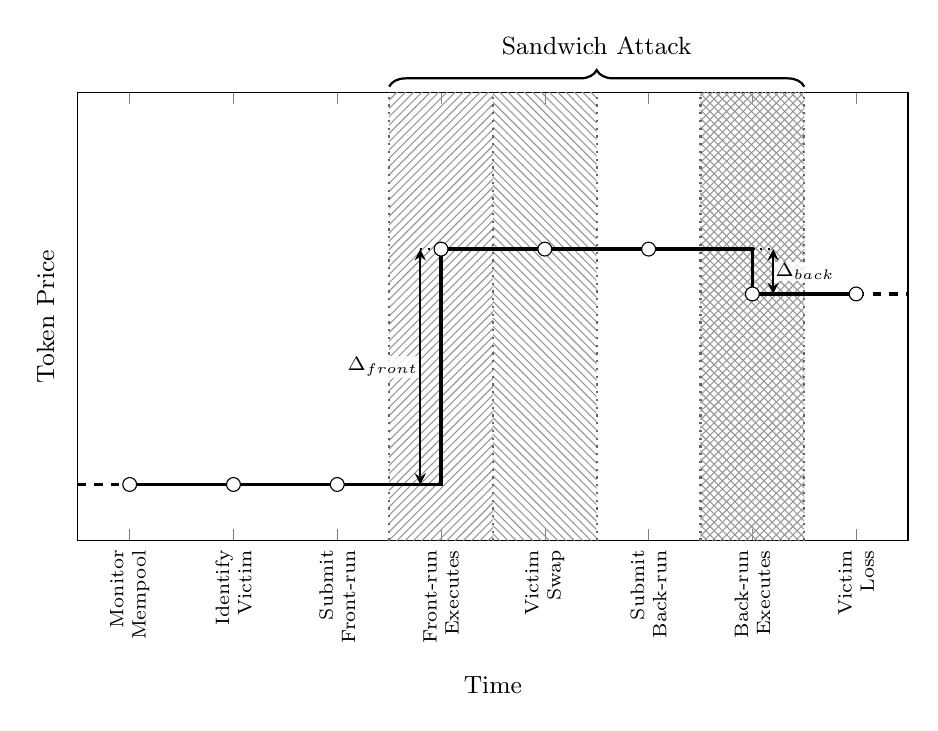
\begin{tikzpicture}
    \begin{axis}[
    % 1. Native sizing
        width=\linewidth,
        height=0.6\linewidth,
        xlabel={Time},
        ylabel={Token Price},
        ymajorgrids=true,
        grid style=dashed,
        xtick={1,2,3,4,5,6,7,8},
        xticklabels={
            Monitor\\Mempool,
            Identify\\Victim,
            Submit\\Front-run,
            Front-run\\Executes,
            Victim\\Swap,
            Submit\\Back-run,
            Back-run\\Executes,
            Victim\\Loss
        },
    % 2. Explicit font sizing
        x tick label style={font=\scriptsize, rotate=90, anchor=east, align=right},
        y tick label style={font=\scriptsize},
    % FIXED: Median spacing (5pt)
        xlabel style={font=\small, yshift=-5pt},
        ylabel style={font=\small, yshift=5pt},
        ymin=0.095,
        ymax=0.135,
        xmin=0.5,
        xmax=8.5,
        ytick=\empty,
        clip=false
    ]


        % --- Hatched Regions ---
        \addplot[pattern=north east lines, pattern color=black!40, draw=none, area legend] coordinates {
            (3.5, 0.095) (4.5, 0.095) (4.5, 0.135) (3.5, 0.135)
        } \closedcycle;

        \addplot[pattern=north west lines, pattern color=black!40, draw=none, area legend] coordinates {
            (4.5, 0.095) (5.5, 0.095) (5.5, 0.135) (4.5, 0.135)
        } \closedcycle;

        \addplot[pattern=crosshatch, pattern color=black!40, draw=none, area legend] coordinates {
            (6.5, 0.095) (7.5, 0.095) (7.5, 0.135) (6.5, 0.135)
        } \closedcycle;

        % --- Separator Lines ---
        \draw[dotted, thick, black!60] (axis cs:3.5, 0.095) -- (axis cs:3.5, 0.135);
        \draw[dotted, thick, black!60] (axis cs:4.5, 0.095) -- (axis cs:4.5, 0.135);
        \draw[dotted, thick, black!60] (axis cs:5.5, 0.095) -- (axis cs:5.5, 0.135);
        \draw[dotted, thick, black!60] (axis cs:6.5, 0.095) -- (axis cs:6.5, 0.135);
        \draw[dotted, thick, black!60] (axis cs:7.5, 0.095) -- (axis cs:7.5, 0.135);

        % --- Price Line Extensions ---
        \addplot[color=black, line width=1.2pt, dashed] coordinates {(0.5, 0.100) (1, 0.100)};
        \addplot[color=black, line width=1.2pt, dashed] coordinates {(8, 0.117) (8.5, 0.117)};

        % --- Price Line ---
        \addplot[color=black, line width=1.2pt, const plot] coordinates {
            (1, 0.100) (2, 0.100) (3, 0.100)
            (4, 0.121) (5, 0.121) (6, 0.121)
            (7, 0.117) (8, 0.117)
        };

        % --- DELTA HIGHLIGHTS (Fixed: fill=white instead of contour) ---
        \draw[<->, >=stealth, thick, black] (axis cs:3.8, 0.100) -- (axis cs:3.8, 0.121)
        node[midway, left, font=\scriptsize, fill=white, inner sep=0.5pt, text opacity=1, fill opacity=0.85] {$\Delta_{front}$};

        \draw[dotted, thick, black] (axis cs:3, 0.100) -- (axis cs:3.8, 0.100);
        \draw[dotted, thick, black] (axis cs:3.8, 0.121) -- (axis cs:4, 0.121);

        \draw[<->, >=stealth, thick, black] (axis cs:7.2, 0.121) -- (axis cs:7.2, 0.117)
        node[midway, right, font=\scriptsize, fill=white, inner sep=0.5pt, text opacity=1, fill opacity=0.85] {$\Delta_{back}$};

        \draw[dotted, thick, black] (axis cs:7, 0.121) -- (axis cs:7.2, 0.121);

        % --- Data Points ---
        \addplot[only marks, mark=*, mark size=2.5pt, color=black, fill=white] coordinates {
            (1, 0.100) (2, 0.100) (3, 0.100)
            (4, 0.121) (5, 0.121) (6, 0.121)
            (7, 0.117) (8, 0.117)
        };

        % --- Curly Bracket ---
        \draw [decorate, decoration={brace, amplitude=6pt, raise=2pt}, thick]
        (axis cs:3.5, 0.135) -- (axis cs:7.5, 0.135)
        node [midway, above=10pt, font=\small] {Sandwich Attack};

    \end{axis}
\end{tikzpicture}

		\caption{Temporal mechanics of a Sandwich Attack. The diagram illustrates the
		eight distinct stages of the attack lifecycle, plotting the Token Price
		evolution against Time. The process begins with the attacker monitoring the mempool
		to identify a pending victim transaction. The attacker subsequently executes
		a front-run transaction, inducing an artificial price increase ($\Delta_{front}$)
		that forces the victim to swap at an inflated rate (slippage). Finally, the attacker
		executes a back-run transaction ($\Delta_{back}$) to close the position and extract
		the price difference as profit.}
		\label{fig:sandwich-attack}
	\end{figure}

	% ii) Existing literature measures the *technical* scope of MEV, but overlooks the *welfare* implications: who actually pays?
	While the technical scope of \ac{MEV} has been extensively documented~\citep{Heimbach2023,Alipanahloo2024,Gramlich2024,Yang2024,Materwala2025,Zhang2025},
	the literature regarding its welfare implications remains sparse. Current discourse
	relies on a limited set of studies: \citet{Appiah2025} estimate a cumulative
	\ac{MEV}-related welfare loss in the hundreds of millions of US dollars~\citep{Appiah2025},
	suggesting a wealth transfer away from users~\citep{Capponi2025} that may disproportionately
	affect retail participants~\citep{FerreiraTorres2021,Guidi2026}. Amidst this
	developing landscape, some have conceptualised these losses as a, potentially illegal,
	\enquote{invisible tax on users}~\citep{Vadlamani2024}, while others position
	\ac{MEV} extraction as an inevitability requiring redistribution rather than
	prevention~\citep{Braga2024}.

	% iii) We provide the first comprehensive audit of the "distributional incidence" of sandwich attacks on Ethereum (2024–2025).
	% iv) Key Finding 1 (Supply): Extraction is highly concentrated (Gini > 0.9), supporting the "Natural Centralization" hypothesis.
	% v) Key Finding 2 (Demand): The burden is regressive; retail traders pay a "stealth tax" orders of magnitude higher per dollar traded than institutional players.

	% Framing
	% i) Frame the paper not as a "crypto study" but as a test of "Market Microstructure Theory" in a novel setting.
	% ii) Position the "billions in extraction" claim carefully: Contrast "Capital at Risk" (Volume Sandwiched) against "Deadweight Loss" (Gas + Slippage) to satisfy economic rigor.
	% iii) Explicitly state the contribution: "We move beyond measuring 'market efficiency' to measuring 'consumer welfare'."

	\section{Institutional Background and Hypothesis Development}
	\label{sec:background-theory}

	\todo[inline]{Place self-cites; hybrid on-chain and off-chain exchanges have some benefits over \ac{DEX}~\citep{Platt2020}; even institutions move more functionality that was traditionally centralised on chain~\citep{KohlLandgraf2025}; retail users misjudge the technological properties of decentralised technology, even if they self-describe as experts~\citep{Platt2023}--an issue that customer education may address~\citep{Dragnoiu2023}; most \acp{L1} are not appropriate for \acp{DEX} due to their low throughput, high latency, high cost, and high energy consumption~\citep{Platt2021}; the need for replication of data amongst distrusting peers has spawned a number of consensus mechanisms~\citep{Platt2023a}, all with different impact on system throughput and latency and, therefore, vulnerability to \ac{MEV}; concerns around privacy of data, including trade data, on public blockchains have been widely discussed~\citep{Platt2021a}.}

	\todo[inline]{Place potential reviewer cites from highly relevant papers; a small group of builders dominate and centralize Ethereum's block-building market~\citep{Wu2025}; the incentives of users and block producers may be balanced by protocol-level mechanisms~\citep{Braga2024b,Fang2025}; block builders tend to collude when they share market conditions, but introducing differences in network latency or enforcing auction deadlines disrupts this behavior~\citep{Wu2024}}

	\todo[inline]{Place potential reviewer cites from target journal; \ac{MEV} constitutes market manipulation that exploits a fragmented regulatory vacuum~\citep{Teng2026}; \ac{MEV} threatens fair price discovery on \ac{DEX}~\citep{Mohan2022}; tick-by-tick data is useful for analyzing crypto markets and attacks like MEV can only be detected using such data~\citep{Anas2024}}

	\subsection{The Block Construction Game as a Priority Auction}
	\label{subsec:block-auction}
	% Key arguments
	% i) Explain the discrete-time nature of blocks vs. continuous-time TradFi markets.
	% ii) Define the "Sandwich" not as a hack, but as a "risk-free" exploitation of ordering privileges (an electronic front-run).

	% Framing
	% i) Use standard auction theory terminology ("First-Price Auctions," "Priority Gas Auctions") to make the mechanism native to RFS readers.

	\subsection{Theoretical Parallels: {HFT} and Latency Arbitrage}
	\label{subsec:hft-parallels}
	% Key arguments
	% i) Draw a direct line to Budish, Cramton, and Shim (2015) regarding high-frequency trading arbitrage.
	% ii) Hypothesis 1: Without regulation, MEV extraction will concentrate into a natural oligopoly due to returns on scale (proprietary signals/latency).
	% iii) Hypothesis 2: Uninformed order flow (retail) will subsidize informed order flow (bots), creating a "Lemons" problem.

	Algorithmic trading, the generation and submission of buy and sell orders by
	an automated system~\citep{Gomber2013}, has gained prominence after 1998, when
	the \ac{SEC} introduced regulations for alternative trading systems~\citep{Goldstein2014}.
	\Ac{HFT} has developed as a result of the 1995--2005 period~\citep{Moallemi2013},
	where implied latency, the time it takes to execute a trade in the market,
	decreased by approximately two orders of magnitude driven by digital
	technology advances and a decline in \ac{ICT} prices~\citep{Zaharudin2021}.

	\citet{Zaharudin2021} explain that latency issues, such as the speed of
	cross-market information flow and transmission speeds across geographical
	locations, are crucial to the success of high-frequency traders and their strategies.
	They mention that eliminating latency arbitrage can reduce the cost of
	liquidity by almost 17\%, suggesting that latency arbitrage is a significant
	and costly market practice. \citet{Aquilina2021} show that latency
	arbitrage arises when the price of an asset changes on one venue, leading to a race
	to capture stale quotes in highly correlated assets or the same asset on other venues,
	and that these races now occur in microseconds or nanoseconds.

	% i) DeFi promises "democratized finance," but the sequential nature of block building introduces a structural vulnerability (MEV) analogous to HFT latency arbitrage.
	\Ac{DeFi} promised to reduce the dependency on centralized intermediaries like banks
	and investment firms, empowering users to interact directly through
	decentralized software applications on peer-to-peer networks~\citep{Bansal2025}.
	Concretely, this was poised to lower counterparty risk, eliminate middlemen, and
	enhance security through automated execution~\citep{Schueffel2021}. Yet,
	as the industry matured, especially after \ac{DeFi} platforms experienced
	exponential growth in liquidity between January 2020 and January 2024~\citep{Durachman2024},
	it became apparent that many functions in \ac{DeFi} mimic \ac{TradFi}, not least
	because many risks that participants in \ac{DeFi} face are exacerbated by
	externalities and information asymmetries which also affect \ac{TradFi}~\citep{Aquilina2021}.

	Both \ac{DeFi} and \ac{TradFi} share fundamentally similar vulnerabilities to
	value-extraction strategies; specifically, the aforementioned \ac{HFT} latency arbitrage
	in \ac{TradFi} is conceptually equivalent to \ac{MEV} in \ac{DeFi}. \ac{MEV}, initially
	termed \textit{miner} extractable value, was formalised in the seminal paper \enquote{Flash Boys 2.0}
	by \citet{Daian2020}. It has been positioned as a technique akin to
	\enquote{front-running} in \ac{TradFi}, wherein traders exploit a speed advantage
	to buy assets just moments before large, institutional block trades drive up
	the price~\citep{Protter2015}, hence the \enquote{Flash Boys}~\citep{Lewis2014}
	analogy. A specific type of \ac{MEV}, focus of this paper, is the \emph{sandwich
	attack}, which involves an attacker strategically positioning profitable
	arbitrage transactions immediately before and after a victim's pending
	transaction to capitalize on the induced price movement, thereby imposing a tax
	on the victim’s trade~\citep{Heimbach2022}.

	\subsection{Hypotheses}
	\label{subsec:hypotheses}

	The parallels above yield five hypotheses, with Hypothesis~\ref{hyp:repeat} explicitly withdrawn in this revised release.

	\begin{hypothesis}[Supply-side concentration]
	\label{hyp:concentration}
	Because success rewards scale -- faster infrastructure and better trading signals -- a small number of searchers capture almost all sandwich-\ac{MEV} volume, yielding a winner-take-most market.
	\end{hypothesis}

	\begin{hypothesis}[Regressive incidence]
	\label{hyp:regressive}
	The sandwich tax is regressive in two conditional senses: (a) \emph{attacked-trade composition} -- observed attack events are concentrated in smaller trade-size tiers relative to attacked notional volume; and (b) \emph{loss incidence} -- modeled loss per dollar traded declines with trade size under alternative scaling assumptions. Part (a) is descriptive composition \(P(\text{trade-size tier}\mid\text{sandwiched})\), not population attack risk \(P(\text{sandwiched}\mid\text{trade-size tier})\); testing part (b) requires either an explicit assumption on per-attack loss scaling or realised-slippage microdata.
	\end{hypothesis}

	\begin{hypothesis}[Persistence]
	\label{hyp:persistence}
	Extraction persists throughout 2024--2025 -- occurring daily and continuing after major protocol upgrades -- rather than being a transitory market failure.
	\end{hypothesis}

	\begin{hypothesis}[Protocol heterogeneity]
	\label{hyp:heterogeneity}
	Sandwich activity differs systematically across \ac{DEX} protocols: a small set of protocols hosts victim trades that are orders of magnitude larger than the market average (\enquote{whale pools}), concentrating the highest-stakes extraction. Protocols here are the twenty \ac{DEX} families on which sandwiched trades appear in our sample -- Uniswap, Curve, Maverick, Balancer, Fluid, PancakeSwap, Ekubo, and thirteen smaller ones -- identified by the \texttt{project} label of the underlying Dune \ac{DEX}-trade tables, with individual liquidity pools and protocol versions aggregated to the protocol level.
	\end{hypothesis}

	\begin{hypothesis}[Repeat victimisation (withdrawn)]
	\label{hyp:repeat}
	This hypothesis is withdrawn in the revised dataset release and is not treated as a confirmed empirical claim in this version.
	\end{hypothesis}

	\todo[inline]{Jana: Please, close this subsection with a short roadmap paragraph mapping each hypothesis to its evidence, so the reader can navigate.}

	\section{Data Construction and Forensic Methodology}
	\label{sec:data-methodology}

	\todo[inline]{Jana}
    Our empirical sample covers 731 consecutive calendar days from 1 January 2024
    to 31 December 2025. The data capture sandwich activity from two complementary
    measurement perspectives: the trading activity of identified sandwich bots and
    the victim transactions affected by these attacks. On the bot side, the sample
    contains 9,917 observed bot addresses and 7,205,506 attacker trade legs,
    representing \$247.52 billion in notional trading volume over the sample period.
    Daily bot-side volume averages \$338.61 million, compared with a median of
    \$276.31 million, and varies substantially over the sample period, from
    \$93.01 million to \$1.61 billion (SD = \$215.99 million). On an average day,
    171.92 active bots execute 9,857 attacker trade legs across 6,610 unique
    transactions. This variation provides the basis for the subsequent analysis
    of changes in sandwich activity over time.
    
    Bot-level activity is highly heterogeneous. Of the 9,917 observed bot
    addresses, 9,800 have measurable USD volume. Mean cumulative volume among
    these bots is \$25.26 million, compared with a median of only \$1,872.10,
    while the largest bot records \$78.08 billion in cumulative volume. Activity
    is similarly skewed: among positive-volume bots, the median bot records
    activity on three distinct days and executes four sandwich trades, compared
    with means of 12.79 days and 735.27 trades, respectively. These large
    differences between the means and medians indicate a strongly right-skewed
    distribution of bot activity, motivating the subsequent analysis of the extent
    to which sandwich activity is concentrated among a relatively small number
    of searchers.
    
    The victim-side data comprise 3,753,857 sandwiched victim transactions and
    \$27.52 billion in victim-side trading volume. Identity counts must be
    distinguished by definition: the taker-based count is 330,521 unique taker
    addresses, while the corrected \texttt{tx\_from} identity layer yields
    742,330 total EOAs (741,404 non-bot trader EOAs). Victim transaction sizes
    average \$7,332.08, compared with a median of \$1,001.85. The 25th and 75th
    percentiles are \$354.97 and \$3,121.76, respectively, while the 90th and
    95th percentiles are \$8,986.61 and \$17,006.16. The observed transaction
    sizes range from a near-zero minimum to a maximum of \$21.01 million. The
    substantial difference between the mean and median, together with the wide
    upper tail of the distribution, indicates considerable heterogeneity in
    victim transaction sizes and motivates examining sandwich exposure separately
    across transaction-size groups.
    
    The victim transactions are further divided into three transaction-size
    groups: Retail, Small, and Institutional. Their construction is described in
    Section~\ref{subsec:trader-classification}. The groups contain 1,876,928
    Retail, 1,501,543 Small, and 375,386 Institutional victim transactions,
    respectively, with average transaction sizes of \$409.84, \$3,082.28, and
    \$58,942.39. These differences provide the basis for the subsequent comparison
    of sandwich exposure and attack frequency across transaction-size groups.
    
    The bot- and victim-side figures represent different measurement bases and are
    therefore reported separately throughout the analysis. Bot-side volume
    aggregates attacker legs associated with sandwich execution, including
    front-running and back-running activity across the DEX pools involved in
    routing, whereas victim-side volume records the sandwiched victim transaction
    itself. Accordingly, the \$247.52 billion in bot-side notional volume and the
    \$27.52 billion in victim-side trading volume represent distinct quantities
    and are treated separately throughout the analysis. The protocol-level data
    provide a further disaggregation of the victim-side sample across 20 DEX
    protocols.
    
    Having established the main characteristics of the sample, we next describe
    the construction of the bot- and victim-side measures, the validation of the
    data, and the empirical procedures used in the subsequent analysis.
    
	\todo[inline]{To do: Natalie}

	\subsection{The 2024–2025 Ethereum Ledger
	Reconstruction}
	\label{subsec:ledger-reconstruction}

	\todo[inline]{To do: Natalie}
    All data are sourced from Dune Analytics, a platform that provides
    real-time indexed access to Ethereum's on-chain records. The sample
    covers 1 January 2024 to 31 December 2025, comprising 731 consecutive
    calendar days. Over this period the dataset records sandwich activity
    involving 3,753,857 victim trades across 9,917 distinct bot
    addresses, with total bot-side sandwiched volume of \$247.52 billion and a daily
    mean of \$338.61 million. No manual data entry was performed; all
    figures are derived directly from SQL queries executed against Dune's
    curated tables, with aggregation performed in SQL only.
    
    Sandwich events are identified using Dune Analytics' curated sandwich
    detection methodology. A sandwich bundle consists of at least three
    transactions appearing in the same block in which the first and last
    transactions share the same initiating address (the bot), both
    interact with the same liquidity pool, and a victim transaction appears
    between them. The victim transaction is the target of the attack:
    it is the trade whose execution price is worsened by the bot's
    front-run~\citep{Daian2020,Heimbach2022}. Each row in the detection
    output therefore represents a victim trade, identified by its
    transaction hash and block number, alongside the addresses of the
    attacking bot and the affected liquidity pool.
    
    Several categories of transaction are excluded from the sample.
    Atomic arbitrages---round-trip trades that begin and end in the same
    token without an identifiable victim---are excluded because they do
    not impose a cost on a counterparty. Transactions that were broadcast
    to the network but reverted on-chain are excluded because no economic
    transfer occurs. Of the 9,917 bot addresses present in the raw data,
    117 have missing USD volume records and are excluded from the
    concentration statistics reported in Section~\ref{sec:supply-side-io},
    though they remain in the attack-count figures. These observations are
    therefore retained in attack-count statistics but excluded from
    calculations based on USD extraction volume.
    
    Token amounts are converted to USD at the block timestamp using Dune
    Analytics' price feed, which draws on liquid \ac{DEX} pools and
    centralised-exchange oracles. For the dominant tokens in the sample
    (ETH, WBTC, USDC, USDT) this conversion is reliable. Long-tail
    tokens traded on smaller protocols may carry price-feed noise;
    however, in the 24-month primary window Uniswap accounts for approximately
    72\% of victim-side notional volume in the protocol table
    (\texttt{query\_protocol\_vulnerability\_v2}). Valuation errors may therefore have a greater
    effect on individual protocols or tokens than on the aggregate event
    count.

	% Key arguments
	% i) Description of the proprietary node infrastructure and dataset (2024–2025).
	% ii) Filtering criteria: How "sandwich bundles" are inextricably linked to victim transactions.

	% Framing
	% i) Emphasize "Curated Data" over "Raw Data." Reviewers value the cleaning process (removing wash trading, atomic arbs) as a signal of quality.

	\subsection{Participant Classification: Identifying the `Uninformed' Trader}
	\label{subsec:trader-classification}
	% Key arguments
	% i) Methodology for the "Retail" vs. "Institutional" split (Quantile-based clustering of transaction size + Wallet age/history).
	% ii) Validation of these clusters against known entities (e.g., CEX hot wallets vs. MetaMask users).

	% Framing
	% i) Frame this as a methodological contribution: "A novel heuristic for on-chain investor classification." This increases citability by other papers needing similar splits.

    Because Ethereum addresses are pseudonymous, the on-chain data do not allow us to directly observe whether a given trader is a retail investor, institutional participant, or another type of market participant. This limitation is common to empirical analyses of activity on public blockchains, where researchers generally rely on observable transaction and address-level characteristics rather than verified investor identities~\citep{FerreiraTorres2021}.

    We therefore classify victim transactions according to their USD trade size and use these groups as a proxy for differences in participant scale. This approach allows us to study whether exposure to sandwich attacks varies systematically with the size of the underlying trade without making claims about the verified identity or wealth of the trader.

    Transaction-level analysis is particularly appropriate in this setting because sandwich attacks arise from the ordering of individual transactions within the blockchain execution environment~\citep{Daian2020,Heimbach2022}. We assign each sandwiched victim transaction to one of three trade-size tiers using exact in-query order-statistic cutoffs. \emph{Retail} transactions are those below \$1,001.85 (\(p_{50}\)); \emph{Small} transactions fall between \$1,001.85 and \$8,986.61 (\(p_{90}\)); and \emph{Institutional} transactions are those at or above \$8,986.61.

    The resulting groups differ substantially in their average transaction size. Mean trade size increases from approximately \$410 for Retail transactions to \$3,082 for Small transactions and \$58,942 for Institutional transactions. This separation provides a basis for examining how the composition of observed attacked trades and conditional repeat-frequency metrics vary with transaction scale.

    The classification is performed at the transaction level rather than the address level, because the sandwich attack is a transaction-level event; the attacker inserts two transactions around a single victim transaction in the same block. A single address may therefore appear in multiple tiers across the sample period. The resulting categories should not be interpreted as mutually exclusive investor types.
    
	\begin{figure}[t]
		\centering
		\tikzsetnextfilename{trade_size_distribution}
\begin{tikzpicture}
    \begin{axis}
        [
        width=0.70\linewidth,
        height=0.45\linewidth,
        xlabel={Victim Tier},
        ylabel={Transaction Size (USD, log\textsubscript{10} scale)},
        xmin=0.5, xmax=3.5,
        ymin=1e-1, ymax=3e7,
        ymode=log,
        log basis y=10,
        xtick={1, 2, 3},
        xticklabels={
                {Retail\\$n=1,876,928$},
                {Small\\$n=1,501,543$},
                {Institutional\\$n=375,386$}
        },
        x tick label style={font=\scriptsize, align=center},
        ytick={0.1, 1, 10, 100, 100000, 1000000, 10000000},
        yticklabels={{0}, {}, {}, {}, {}, {}, {10,000,000}},
        y tick label style={font=\scriptsize},
        ylabel style={font=\small, yshift=5pt},
        xlabel style={font=\small, yshift=-5pt},
        tick label style={font=\scriptsize},
        % Grid: horizontal lines only (y-axis)
        y grid style={dashed, black!30},
        x grid style={draw=none},
        grid=major,
        axis lines=left,
        title={Trade Size Distribution by Victim Tier (2024-2025)},
        title style={font=\normalsize\bfseries, yshift=10pt},
        clip mode=individual,
        clip=true
        ]

        % Hatched area from brace to y-axis (drawn first, so it's behind everything)
        % Rectangle from y-axis (x=0.5) to brace position (x=3.5), spanning the range
        \fill[
            pattern=north east lines,
            pattern color=black!15,
            draw=none
        ] (axis cs:0.5, 409.84) rectangle (axis cs:3.5, 58942.39);

        % Dotted lines from top and bottom of brace to y-axis (drawn first, so behind everything)
        \draw[
            dotted,
            line width=0.8pt,
            color=black
        ] (axis cs:3.5, 409.84) -- (axis cs:0.5, 409.84);
        \draw[
            dotted,
            line width=0.8pt,
            color=black
        ] (axis cs:3.5, 58942.39) -- (axis cs:0.5, 58942.39);

        % Tier boundary indicators (drawn early so behind violins)
        % Boundary between Retail and Small: p50 = 1001.85
        \draw[
            line width=0.8pt,
            color=black!70,
            dash pattern=on 4pt off 2pt on 1pt off 2pt
        ] (axis cs:0.5, 1001.85) -- (axis cs:3.5, 1001.85);
        % Add a small vertical marker on the y-axis
        \draw[
            line width=0.8pt,
            color=black
        ] (axis cs:0.5, 1001.85) -- (axis cs:0.48, 1001.85);
        \node[
            anchor=east,
            font=\scriptsize,
            text=black,
            fill=white,
            inner sep=2pt,
            xshift=-5pt
        ] at (axis cs:0.5, 1001.85) {1,002};

        % Boundary between Small and Institutional: p90 = 8,986.61
        \draw[
            line width=0.8pt,
            color=black!70,
            dash pattern=on 4pt off 2pt on 1pt off 2pt
        ] (axis cs:0.5, 8986.61) -- (axis cs:3.5, 8986.61);
        % Add a small vertical marker on the y-axis
        \draw[
            line width=0.8pt,
            color=black
        ] (axis cs:0.5, 8986.61) -- (axis cs:0.48, 8986.61);
        \node[
            anchor=east,
            font=\scriptsize,
            text=black,
            fill=white,
            inner sep=2pt,
            xshift=-5pt
        ] at (axis cs:0.5, 8986.61) {8,987};

        % Retail Violin (dark crosshatch)
        \addplot[
            pattern=crosshatch,
            pattern color=black!60,
            draw=black,
            line width=0.8pt,
            fill opacity=1
        ] table[
        x=x,
        y=y,
        col sep=comma
        ] {trade_size_distribution_data_retail.csv};

        % Small Violin (dark crosshatch)
        \addplot[
            pattern=crosshatch,
            pattern color=black!60,
            draw=black,
            line width=0.8pt,
            fill opacity=1
        ] table[
        x=x,
        y=y,
        col sep=comma
        ] {trade_size_distribution_data_small.csv};

        % Institutional Violin (dark crosshatch)
        \addplot[
            pattern=crosshatch,
            pattern color=black!60,
            draw=black,
            line width=0.8pt,
            fill opacity=1
        ] table[
        x=x,
        y=y,
        col sep=comma
        ] {trade_size_distribution_data_institutional.csv};

        % Mean markers: small black 45-degree rotated squares at the mean of each violin
        \node[fill=black, draw=black, line width=0.5pt, shape=rectangle, minimum size=4pt, rotate=45, inner sep=0pt] at (axis cs:1, 409.84) {};
        \node[fill=black, draw=black, line width=0.5pt, shape=rectangle, minimum size=4pt, rotate=45, inner sep=0pt] at (axis cs:2, 3082.28) {};
        \node[fill=black, draw=black, line width=0.5pt, shape=rectangle, minimum size=4pt, rotate=45, inner sep=0pt] at (axis cs:3, 58942.39) {};

        % Annotations: Mean values above each violin
        % Position at 1.5x above the maximum height of each violin (max_tx * 1.5)
        \node[
            anchor=south,
            font=\small,
            text=black,
            fill=white,
            fill opacity=0.8,
            draw=black,
            line width=0.5pt,
            inner sep=3pt
        ] at (axis cs:1, 1502.77) {$\mu = 410$};

        \node[
            anchor=south,
            font=\small,
            text=black,
            fill=white,
            fill opacity=0.8,
            draw=black,
            line width=0.5pt,
            inner sep=3pt
        ] at (axis cs:2, 13479.92) {$\mu = 3,082$};

        \node[
            anchor=south,
            font=\small,
            text=black,
            fill=white,
            fill opacity=0.8,
            draw=black,
            line width=0.5pt,
            inner sep=3pt
        ] at (axis cs:3, 31508190) {$\mu = 58,942$};

        % Range indicator: vertical bracket on the right side
        % Connect Retail mean to Institutional mean
        \draw[
            decoration={brace, amplitude=10pt, mirror},
            decorate,
            line width=0.8pt,
            color=black
        ] (axis cs:3.5, 409.84) -- (axis cs:3.5, 58942.39);
        % Label aligned with brace apex (midpoint) - adjusted y position to account for text baseline
        \node[
            anchor=west,
            font=\small,
            text=black,
            xshift=8pt,
            yshift=-2pt
        ] at (axis cs:3.5, 29676.12) {143.8$\times$ spread};

    \end{axis}
\end{tikzpicture}

		\caption{Trade Size Distribution by Victim Tier (2024-2025). Violin plots show
		the empirical distribution from query5d for Retail ($<$\$1{,}001.85, $\mu=\$410$),
			Small (\$1{,}001.85--\$8{,}986.61, $\mu=\$3{,}082$), and Institutional ($\geq$\$8{,}986.61, $\mu=\$58{,}942$) tiers. Each violin
			displays the mean (black diamond marker). The distribution spans a 143.8$\times$ spread in mean trade size across
tiers, motivating the three-way classification used throughout the analysis.}
		\label{fig:trade-size-distribution}
	\end{figure}

	\subsection{Empirical Strategy}
	\label{subsec:empirical-strategy}
	% Key arguments
	% i) Plain-language description of the estimators and inference used in the results sections (trend regressions with HAC errors, clustered-SE robustness, bootstrap, permutation tests, Poisson rate ratios).
	% ii) Reproducibility: all results generated by a scripted pipeline; every number traceable to a table or report artefact.

	\todo[inline]{Jana: Please, draft this subsection as a plain-language guide to the estimators used in the results sections, so a reader without an econometrics background can follow.}

	\section{Aggregate Estimates of Welfare Extraction}
	\label{sec:aggregate-welfare}

	\subsection{Total Volume at Risk vs. Realized Extraction}
	\label{subsec:volume-vs-extraction}
	% Key arguments
	% i) Present the "Low single-digit billions" figure as "Total Volume Sandwiched" (Capital exposed to manipulation).
	% ii) Decompose the cost: "Gross Profit" (Searcher Revenue) vs. "Network Deadweight Loss" (Gas Fees + Validator Tips).

	% Framing
	% i) This nuanced breakdown protects you from attacks on the "profitability" decline. Even if bot *profits* are down, the *cost to the network* (welfare loss) remains high due to competitive bidding (tips).

	\begin{figure}[t]
		\centering
		\tikzsetnextfilename{temporal_stability}
\begin{tikzpicture}
    \begin{axis}[
        width=\linewidth,
        height=0.5\linewidth,
        xlabel={Date},
        ylabel={Daily Sandwich Volume (\$M, log scale)},
        xmin=0, xmax=730,
        ymin=10, ymax=2000,
        ymode=log,
        log basis y=10,
        grid=major,
        grid style={dashed, black!20},
        axis lines=left,
        xlabel style={font=\small, yshift=-5pt},
        ylabel style={font=\small, xshift=-5pt},
        tick label style={font=\scriptsize},
        xtick={0, 91, 182, 273, 365, 456, 547, 638, 730},
        xticklabels={
            Jan 2024,
            Apr 2024,
            Jul 2024,
            Oct 2024,
            Jan 2025,
            Apr 2025,
            Jul 2025,
            Oct 2025,
            Dec 2025
        },
        x tick label style={font=\scriptsize, rotate=45, anchor=north east},
        ytick={10, 50, 100, 200, 500, 1000, 2000},
        yticklabels={10, 50, 100, 200, 500, 1000, 2000},
        legend style={
            at={(0.98,0.02)},
            anchor=south east,
            font=\scriptsize,
            cells={align=left},
            legend plot pos=left
        },
        clip=false
    ]
        
        % 95% Confidence Band (shaded area)
        \addplot[
            name path=ci_upper,
            draw=none
        ] table[
            x=days_since_start,
            y=ci_upper,
            col sep=comma
        ] {temporal_stability_data.csv};
        
        \addplot[
            name path=ci_lower,
            draw=none
        ] table[
            x=days_since_start,
            y=ci_lower,
            col sep=comma
        ] {temporal_stability_data.csv};
        
        \addplot[
            draw=none,
            pattern=north east lines,
            pattern color=black!50
        ] fill between[
            of=ci_upper and ci_lower
        ];
        
        % 7-day Moving Average (main line)
        \addplot[
            color=black,
            line width=1.2pt,
            mark=none
        ] table[
            x=days_since_start,
            y=ma7,
            col sep=comma
        ] {temporal_stability_data.csv};
        \addlegendentry{7-day MA}
        
        % Mean daily volume horizontal line
        \addplot[
            color=black,
            line width=0.5pt,
            dashed,
            legend image post style={dashed, line width=0.5pt}
        ] coordinates {(0, 338.3) (730, 338.3)};
        \addlegendentry{Mean}
        
        % Mean label on the right, aligned with the line
        \node[
            anchor=west,
            font=\tiny,
            text=black
        ] at (axis cs:730, 338.3) {Mean};
        
        % Vertical markers for major events
        % Dencun upgrade: March 13, 2024 (day 72)
        \draw[
            color=black,
            line width=0.8pt,
            dotted
        ] (axis cs:72, 10) -- (axis cs:72, 2000);
        \node[
            anchor=west,
            font=\tiny,
            text=black,
            rotate=90
        ] at (axis cs:72, 2000) {Dencun};
        
        % Pectra upgrade: May 7, 2025 (day 492)
        \draw[
            color=black,
            line width=0.8pt,
            dotted
        ] (axis cs:492, 10) -- (axis cs:492, 2000);
        \node[
            anchor=west,
            font=\tiny,
            text=black,
            rotate=90
        ] at (axis cs:492, 2000) {Pectra};
        
    \end{axis}
\end{tikzpicture}

		\caption{Persistence of daily sandwich volume (2024--2025). The plot shows
			daily sandwich-attack volume (log scale) with its 7-day centred moving average,
			markers for the Dencun (13 March 2024) and Pectra (7 May 2025) upgrades, and the
			sample mean. Volume is positive on all 731 days, never falling below \$93.0M and
			averaging \$338.61M per day.}
		\label{fig:temporal-stability}
	\end{figure}

	\subsection{Protocol Heterogeneity: The Rise of `Whale Pools'}
	\label{subsec:protocol-heterogeneity}
	% Key arguments
	% i) Empirical breakdown of MEV volume by DEX (Uniswap vs. Ekubo/Maverick).
	% ii) Finding: Newer, capital-efficient AMMs (Ekubo) attract larger trade sizes, acting as "honeypots" for deeper extraction.

	% Framing
	% i) Frame as "The unintended consequences of innovation." More efficient DEX designs (concentrated liquidity) may inadvertently increase the attack surface for predatory pricing.

	Router-intermediation diagnostics indicate that a substantial share of victim-side events are routed through high-throughput contract takers rather than direct trader addresses. In the revised 24-month window, the top 30 taker contracts by distinct senders account for 53.85\% of all victim trades. This implies that protocol-level heterogeneity in observed trade sizes can partly reflect access-path composition (router-fronted vs. direct flow), not only differences in trader capital. We therefore interpret protocol-level size differences as a joint outcome of venue characteristics and intermediation structure.

	\section{The Industrial Organization of MEV (Supply Side)}
	\label{sec:supply-side-io}

	\subsection{Searcher Concentration and Natural Oligopoly}
	\label{subsec:searcher-concentration}
	% Key arguments
	% i) Lorenz Curve and Gini Coefficient analysis of bot revenues.
	% ii) The "Super-Searcher" phenomenon: The top decile controls the market.

	% Framing
	% i) Direct validation of Azar et al. (2024) "Natural Centralization." Use the phrase: "We find empirical support for the hypothesis that MEV markets tend toward natural monopoly."

	\begin{figure}[t]
		\centering
		\tikzsetnextfilename{lorenz_curve}
\begin{tikzpicture}
    \begin{axis}[
        width=\linewidth,
        height=0.45\linewidth,
        xlabel={Cumulative \% of Bots},
        ylabel={Cumulative \% of Volume},
        xmin=0, xmax=100,
        ymin=0, ymax=100,
        grid=major,
        grid style={dashed, black!20},
        axis lines=left,
        xlabel style={font=\small, yshift=-5pt},
        ylabel style={font=\small, xshift=-5pt},
        tick label style={font=\scriptsize},
        legend style={
            at={(0.98,0.02)},
            anchor=south east,
            font=\scriptsize,
            cells={align=left}
        },
        clip=false
    ]
        
        % Perfect Equality line (45° diagonal, dashed)
        \addplot[
            name path=perfect_equality,
            color=black!50,
            line width=1pt,
            dashed,
            domain=0:100
        ] {x};
        \addlegendentry{Perfect Equality}
        
        % Lorenz curve data (thick black line)
        \addplot[
            name path=lorenz_curve,
            color=black,
            line width=1.5pt,
            smooth,
            mark=none
        ] table[
            x=cumulative_pct_bots,
            y=cumulative_pct_volume,
            col sep=comma
        ] {lorenz_data.csv};
        \addlegendentry{Data}
        
        % Hatched area between perfect equality and Lorenz curve (Gini coefficient)
        \addplot[
            draw=none,
            pattern=north east lines,
            pattern color=black!25
        ] fill between[
            of=perfect_equality and lorenz_curve
        ];
        
        % Annotation: "Top 1% controls 98.5%" arrow at 99% x-axis
        \draw[->, >=stealth, color=black!70, line width=0.8pt] 
            (axis cs:99, 98.5) -- (axis cs:99, 92);
        \node[
            anchor=north,
            font=\scriptsize,
            text=black,
            align=center
        ] at (axis cs:99, 90.5) {Top 1\% controls\\98.5\%};
        
        % Annotation: "Gini = 0.998" in shaded region
        \node[
            anchor=center,
            font=\small,
            text=black,
            fill=white,
            fill opacity=0.8,
            inner sep=3pt,
            rounded corners=2pt
        ] at (axis cs:50, 25) {Gini = 0.998};
        
    \end{axis}
\end{tikzpicture}

		\caption{Lorenz Curve showing the distribution of MEV extraction volume
		across bots. The diagonal dashed line represents perfect equality, while the
		blue curve shows the actual distribution. The shaded area between these lines
		represents the Gini coefficient (0.998), indicating extreme concentration: the
		top 1\% of bots control 98.5\% of the total volume.}
		\label{fig:lorenz-curve}
	\end{figure}

	\subsection{Entry, Longevity, and Turnover of Searchers}
	\label{subsec:searcher-dynamics}
	% Key arguments
	% i) Longevity and activity intensity of bots; volume share of persistent vs. transient addresses.
	% ii) Cohorts by first appearance; fewer, larger bots over time (declining daily active bots, rising volume per bot).

	\section{Distributional Incidence of the Stealth Tax (Demand Side)}
	\label{sec:demand-side-incidence}

	\subsection{Regressive Taxation: Retail vs. Institutional Burdens}
	\label{subsec:regressive-tax}
	% Key arguments
	% i) The core "RFS Result": >50% of victims are small (<$10k), but they provide a disproportionate share of "easy" profits relative to volume.
	% ii) Institutional traders effectively "opt-out" via RFQ/Private RPCs; retail does not.

	% Framing
	% i) Use "Taxation" analogies. "Effective Spread" analysis showing that MEV acts as a 10-30bps additional tax on retail, while institutions pay near-zero MEV tax.

	\begin{figure}[t]
		\centering
		\tikzsetnextfilename{victim_impact_metrics}
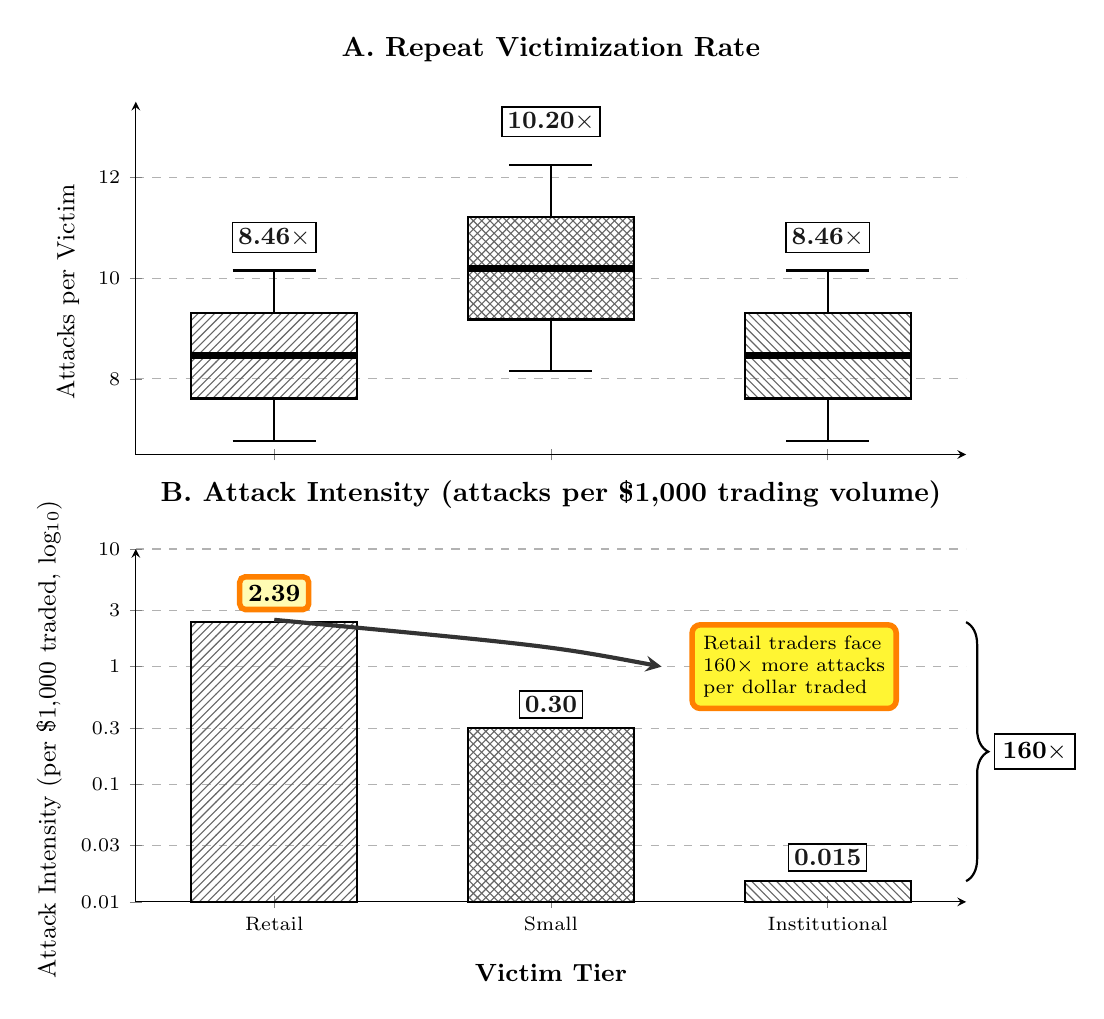
\begin{tikzpicture}
    \begin{groupplot}[
        group style={
            group size=1 by 2,
            vertical sep=1.2cm,
            x descriptions at=edge bottom
        },
        width=\linewidth,
        height=0.5\linewidth,
        xmin=0.5, xmax=3.5,
        xtick={1, 2, 3},
        xticklabels={Retail, Small, Institutional},
        x tick label style={font=\scriptsize, align=center},
        axis lines=left,
        tick label style={font=\scriptsize},
        y grid style={dashed, black!30},
        x grid style={draw=none},
        grid=major,
        clip=false
    ]
    
    % ========================================
    % PANEL A: Repeat Victimization Rate
    % ========================================
    \nextgroupplot[
        ylabel={Attacks per Victim},
        ylabel style={font=\small, xshift=-5pt},
        ymin=6.5, ymax=13.5,
        title={A. Repeat Victimization Rate},
        title style={font=\normalsize\bfseries, yshift=5pt}
    ]
    
    % Retail box plot
    \fill[pattern=north east lines, pattern color=black!60, draw=black, line width=0.8pt] 
        (axis cs:0.7, 7.61) rectangle (axis cs:1.3, 9.31);
    \draw[line width=2.5pt, color=black] (axis cs:0.7, 8.46) -- (axis cs:1.3, 8.46);
    \draw[line width=0.8pt, color=black] (axis cs:1.0, 6.77) -- (axis cs:1.0, 7.61);
    \draw[line width=0.8pt, color=black] (axis cs:0.85, 6.77) -- (axis cs:1.15, 6.77);
    \draw[line width=0.8pt, color=black] (axis cs:1.0, 9.31) -- (axis cs:1.0, 10.15);
    \draw[line width=0.8pt, color=black] (axis cs:0.85, 10.15) -- (axis cs:1.15, 10.15);
    \node[anchor=south, font=\small\bfseries, text=black, fill=white, fill opacity=0.9, draw=black, line width=0.5pt, inner sep=2pt] 
        at (axis cs:1.0, 10.5) {8.46$\times$};
    
    % Small box plot
    \fill[pattern=crosshatch, pattern color=black!60, draw=black, line width=0.8pt] 
        (axis cs:1.7, 9.18) rectangle (axis cs:2.3, 11.22);
    \draw[line width=2.5pt, color=black] (axis cs:1.7, 10.20) -- (axis cs:2.3, 10.20);
    \draw[line width=0.8pt, color=black] (axis cs:2.0, 8.16) -- (axis cs:2.0, 9.18);
    \draw[line width=0.8pt, color=black] (axis cs:1.85, 8.16) -- (axis cs:2.15, 8.16);
    \draw[line width=0.8pt, color=black] (axis cs:2.0, 11.22) -- (axis cs:2.0, 12.24);
    \draw[line width=0.8pt, color=black] (axis cs:1.85, 12.24) -- (axis cs:2.15, 12.24);
    \node[anchor=south, font=\small\bfseries, text=black, fill=white, fill opacity=0.9, draw=black, line width=0.5pt, inner sep=2pt] 
        at (axis cs:2.0, 12.8) {10.20$\times$};
    
    % Institutional box plot
    \fill[pattern=north west lines, pattern color=black!60, draw=black, line width=0.8pt] 
        (axis cs:2.7, 7.61) rectangle (axis cs:3.3, 9.31);
    \draw[line width=2.5pt, color=black] (axis cs:2.7, 8.46) -- (axis cs:3.3, 8.46);
    \draw[line width=0.8pt, color=black] (axis cs:3.0, 6.77) -- (axis cs:3.0, 7.61);
    \draw[line width=0.8pt, color=black] (axis cs:2.85, 6.77) -- (axis cs:3.15, 6.77);
    \draw[line width=0.8pt, color=black] (axis cs:3.0, 9.31) -- (axis cs:3.0, 10.15);
    \draw[line width=0.8pt, color=black] (axis cs:2.85, 10.15) -- (axis cs:3.15, 10.15);
    \node[anchor=south, font=\small\bfseries, text=black, fill=white, fill opacity=0.9, draw=black, line width=0.5pt, inner sep=2pt] 
        at (axis cs:3.0, 10.5) {8.46$\times$};
    
    % ========================================
    % PANEL B: Attack Intensity
    % ========================================
    \nextgroupplot[
        ylabel={Attack Intensity (per \$1,000 traded, log\textsubscript{10})},
        ylabel style={font=\small, xshift=-5pt},
        ymode=log,
        log basis y=10,
        ymin=0.01, ymax=10,
        ytick={0.01, 0.03, 0.1, 0.3, 1, 3, 10},
        yticklabels={0.01, 0.03, 0.1, 0.3, 1, 3, 10},
        xlabel={Victim Tier},
        xlabel style={font=\small\bfseries, yshift=-5pt},
        title={B. Attack Intensity (attacks per \$1,000 trading volume)},
        title style={font=\normalsize\bfseries, yshift=5pt}
    ]
    
    % Retail bar
    \fill[pattern=north east lines, pattern color=black!60, draw=black, line width=0.8pt] 
        (axis cs:0.7, 0.01) rectangle (axis cs:1.3, 2.39);
    \node[anchor=south, font=\small\bfseries, text=black, fill=yellow!30, draw=orange, line width=2pt, inner sep=3pt, rounded corners=2pt] 
        at (axis cs:1.0, 2.9) {2.39};
    
    % Small bar
    \fill[pattern=crosshatch, pattern color=black!60, draw=black, line width=0.8pt] 
        (axis cs:1.7, 0.01) rectangle (axis cs:2.3, 0.30);
    \node[anchor=south, font=\small\bfseries, text=black, fill=white, fill opacity=0.9, draw=black, line width=0.5pt, inner sep=2pt] 
        at (axis cs:2.0, 0.36) {0.30};
    
    % Institutional bar
    \fill[pattern=north west lines, pattern color=black!60, draw=black, line width=0.8pt] 
        (axis cs:2.7, 0.01) rectangle (axis cs:3.3, 0.015);
    \node[anchor=south, font=\small\bfseries, text=black, fill=white, fill opacity=0.9, draw=black, line width=0.5pt, inner sep=2pt] 
        at (axis cs:3.0, 0.018) {0.015};
    
    % Annotation 1: Regressive Pattern Callout
    \draw[->, >=stealth, color=black!80, line width=1.5pt, bend left=15] 
        (axis cs:1.0, 2.5) .. controls (axis cs:2.0, 1.5) .. (axis cs:2.4, 1.0);
    \node[anchor=west, font=\scriptsize, text=black, fill=yellow!80, draw=orange, line width=2pt, inner sep=4pt, rounded corners=3pt, align=left] 
        at (axis cs:2.5, 1.0) {Retail traders face\\160$\times$ more attacks\\per dollar traded};
    
    % Annotation 2: Ratio Bracket
    \draw[decoration={brace, amplitude=8pt, mirror}, decorate, line width=0.8pt, color=black] 
        (axis cs:3.5, 0.015) -- (axis cs:3.5, 2.39);
    \node[anchor=west, font=\small\bfseries, text=black, fill=white, draw=black, line width=0.5pt, inner sep=3pt] 
        at (axis cs:3.6, 0.19) {160$\times$};
    
    \end{groupplot}
\end{tikzpicture}

		\caption{Victim Impact Metrics. (A) Using non-bot \texttt{tx\_from} identity in query5c, Small traders face higher mean attack frequency than Retail traders (5.40 vs.\ 4.76 attacks per trader EOA), while the median in every tier equals 1. (B) Attack intensity per \$1,000 traded is mechanically proportional to inverse mean trade size; in this window Retail exceeds Institutional by 143.8$\times$. Data: 3,753,857 sandwich attacks, 2024--2025.}
		\label{fig:victim-impact-metrics}
	\end{figure}

	\subsection{Repeat Victimization and Capital Erosion (Withdrawn)}
	\label{subsec:repeat-victimization}
	% Key arguments
	% i) Analysis of "Attack Frequency per Dollar Traded."
	% ii) Retail addresses are "habitual victims," suggesting a lack of learning or tool access (sticky technology).

	% Framing
	% i) This is a "Consumer Protection" argument. It counters the "efficient market" view that traders will naturally adapt to avoid predation. They don't (or can't).

	This subsection is retained for structure only; the repeat-victimisation hypothesis is withdrawn and not used as a load-bearing claim.

	\section{Robustness Checks and Limitations}
	\label{sec:robustness}

	\todo[inline]{To do: Natalie}

    Our sandwich-detection records are generated by Dune Analytics'
    curated detection methodology, which identifies attacks routed through
    Ethereum's public mempool. Attacks submitted through private
    transaction-ordering mechanisms may therefore not be captured. All
    volume and count figures should consequently be interpreted as
    conservative estimates of observed sandwich activity. The extent of
    this undercount may also vary over time as the use of private
    transaction-ordering mechanisms changes over the sample period.
    
    The \$247.52B headline figure measures capital \emph{exposed} to
    sandwiching, not capital lost. Converting exposure to realised victim
    loss requires slippage decomposition at the trade level---the
    difference between the victim's execution price and the counterfactual
    fair price---which is not available in our aggregated data. Our volume
    figures should therefore be interpreted as measures of exposure to
    sandwich attacks rather than direct estimates of economic harm or
    welfare loss.
    
    USD valuations rely on Dune's price feed, sourced from liquid
    \ac{DEX} pools and centralised-exchange oracles at the relevant block
    timestamp. For the dominant tokens in our sample (ETH, WBTC, USDC,
    USDT), valuation error is likely to be limited. Long-tail tokens
    traded on smaller protocols may carry price-feed noise, although
    in the 24-month primary window, Uniswap accounts for approximately 72\%
    of victim-side notional volume in \texttt{query\_protocol\_vulnerability\_v2}. Such valuation error may therefore have a greater
    effect on individual protocols or tokens than on the aggregate event
    count.
    
    Ethereum addresses are pseudonymous: a single operator may control
    multiple bot wallets, so our count of 9,917 bot addresses should not
    be interpreted as the number of independent searchers. Similarly,
    victim tier labels classify individual \emph{trades} by size, not
    traders by identity; a single address may appear in multiple tiers
    across the sample period.
    
    Finally, protocol-level sandwich volumes in
    Section~\ref{subsec:protocol-heterogeneity} are reported as absolute
    figures. Without each protocol's total trading volume over the same
    period, we cannot compute a sandwich \emph{rate}; high-volume
    protocols therefore appear more exposed by construction. Normalisation
    by protocol-level trading volume is left for future work as
    protocol-wide volume data become available.

	% Key arguments
	% i) Does high gas price volatility drive the results? (Controls included).
	% ii) Are these just "bad trades" (high slippage settings) or actual attacks? (Slippage controls).
	% iii) Limitation: Off-chain agreements/private order flow not fully visible (conservative lower bound).

	% Framing
	% i) Essential for RFS acceptance. Anticipate the reviewer's doubt: "Is this just user error?" Prove it is structural predation.

	\section{Policy Implications and Market Design}
	\label{sec:policy-implications}

	\subsection{MEV as Market Abuse under MAR and MiCA}
	\label{subsec:regulatory-implications}
	% Key arguments
	% i) Map findings to the UK FCA's "Market Abuse" definitions (DP24/4).
	% ii) Argument: If retail cannot avoid the tax, it violates "Treating Customers Fairly" (TCF) principles.

	% Framing
	% i) Increases impact/citability by policy papers. explicitly state: "Sandwiching meets the economic definition of front-running, distinct from arbitrage."

	\subsection{Designing for Fairness: Batch Auctions and Privacy}
	\label{subsec:market-design}
	% Key arguments
	% i) Brief discussion of solutions: Encrypted mempools, Batch auctions (CowSwap).
	% ii) Economic trade-off: Latency vs. Fairness.

	% Framing
	% i) Ends on a constructive, forward-looking note, which is typical for top-tier finance journals.

	\section{Conclusion}
	\label{sec:conclusion}

	% Key arguments
	% i) Summarize: MEV is not just a security cost; it is a distributional issue.
	% ii) Final thought: Sustainable DeFi adoption requires solving the "Stealth Tax" on the smallest users.

	% Framing
	% i) Reiterate the "Inequality" angle. This is the lasting takeaway that gets cited in broader economic literature.

	\bibliography{references}
\end{document}